\documentclass{article}
\usepackage[left = 25.4mm,right = 25.4mm,top = 25.4mm,bottom = 25.4mm]{geometry}
\usepackage{setspace}
\usepackage{graphicx}
\usepackage{hyperref}
\usepackage{indentfirst}
\usepackage[utf8]{inputenc}
\usepackage{biblatex}
\usepackage{amsmath}
\usepackage{authblk}
\usepackage{datetime}

\addbibresource{bib.bib}
%\doublespacing
\graphicspath{ {./images/} }
\setlength{\parindent}{2em}

\title{\Huge Project: Photodiode IR Amplification Circuit}
\begin{document}
\date{April 22, 2021}
\author{Christopher Lemus
  \thanks{Electronic address: \texttt{lemusc@bu.edu}}}
\affil{Department of Electrical Engineering, Boston University}
\maketitle

\section{Purpose}
\indent The purpose of this project is to utilize concepts learned from analog electronics and apply them to a project of our own. In the case of this report, a photodiode amplification circuit was created using BJTs. 

\section{Introduction}
\indent This is a great project to work on because the world is governed by data which is collected from hundreds of thousands of sensors in a system. For example, the stresses on a length of metal can be calculated accurately by using a sensor (namely a strain gauge) which is able to change resistance proportional to the strain it undergoes. These signals can be very small most of the time - and this is where the amplification of the signal comes in. The application of a circuit like this can be extended to audio signals as well - and work well if the stages are coupled correctly.\par 
\indent The schematic of the circuit is shown below in Figure 1 along with resistor values that were used in the real physical prototype. The values of each node will be calculated in Section 4 - Data Analysis so we can conclude the overall gain of the circuit.
\begin{figure}[h!]
\centering
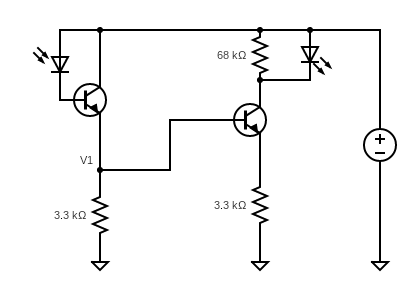
\includegraphics[width=0.8\textwidth]{circuit (1).png}
\caption{{Photodiode Circuit}}
\end{figure}

\section{Procedure/Materials}
\indet This section is intended to provide the components which were used and the values which were used as well:
\begin{enumerate}
    \item 2 NPN 2N2222 BJTs
    \item 1 Photodiode
    \item 1 LED (preferably InGaN) 
    \item 1 68k$\Omega$ Resistor
    \item 2 3.3k$\Omega$ Resistor2
    \item 9V Positive Voltage Source & Ground or 9V Battery
\end{enumerate}
\indent The procedure to completing a replica of this circuit will be described. Construct the circuit in Figure 1. Note that a power supply of +9V was used. \par 
\indet Here is an important note. All LEDs of different colors require different forward voltage $V_f$ in order to properly function. For example red LEDs are the easiest to turn on because they require a forward voltage of 2.0 V. In this circuit a cool white LED of Indium Gallium Nitride (InGaN) was used - which requires a $V_f$ of 3.3 V to begin emission. Therefore, if you decide to change around values, ensure that you have a proper LED otherwise you run the risk of having the LED on the entire time even under Zero sources of infrared light (which the Photodiode will pick up). 
\section{Data}
\indent Although I do not posses a Lumen detector to plot the LED output as a function of distance I can provide observations from operating the Photodiode circuit. The circuit works very well at picking up IR light from fire and IR light from IR blasters which our phones which use for Face ID. When aiming a remote control at the Photodiode we also get a very good response which proves that this is a very practical device (and as we will see later can be made into a very user friendly size). As long as the sources of IR are in the direct line-of-action of the Photodiode then the LED will become operational. The exciting part is when you begin adding distance between the Photodiode and IR source. As long as you keep the source in the line of line-of-action of the Photodiode then you will get a response. When aiming my iPhone with the screen on at the Photodiode I can get a response up through my wingspan. When using a lighter or candle I can get a response from the circuit at up to a meter. The biggest obstacle with testing this circuit is being able to get the source lined up with the Photodiode so that it can turn on. 

\section{Data Analysis}
\indent Under a source the Photodiode will generate a 300mV signal. The goal is to amplify this enough so that we can get the LED to turn on and emit brighter as the intensity of the source increases. The LED at the collector of the second stage forces the collector current to remain very small about 10$\mu$A. If the Photodiode is generating a peak voltage of 300 mV then we can use KVL and say 9v - 0.300v - 0.650v = $V_1$, which is approximately 8.05V. At the second stage we take the 8.05V from the emitter of stage 1 and subtract 0.65v for the second transistor and we find that the second stage 3.3k$\Omega$ resistor must dissipate 7.4V. Therefore the emitter current is approximately 2.2 mA and dependant on the Photodiode and its reception of the IR source. \par
\indent Figure 2 shows the output of current through the 68k$\Omega$ resistor, which is significant because this is the forward voltage of the LED. The LED will increase in intensity as the Photodiode absorbs more IR light and causes an increase in the diode current in the second stage. \par
\indet The gain of the second stage is $\frac{68}{3.3}$ = 20.6. This is enough to achieve the voltage required to enable emission of the LED.
\begin{figure}[h!]
\centering
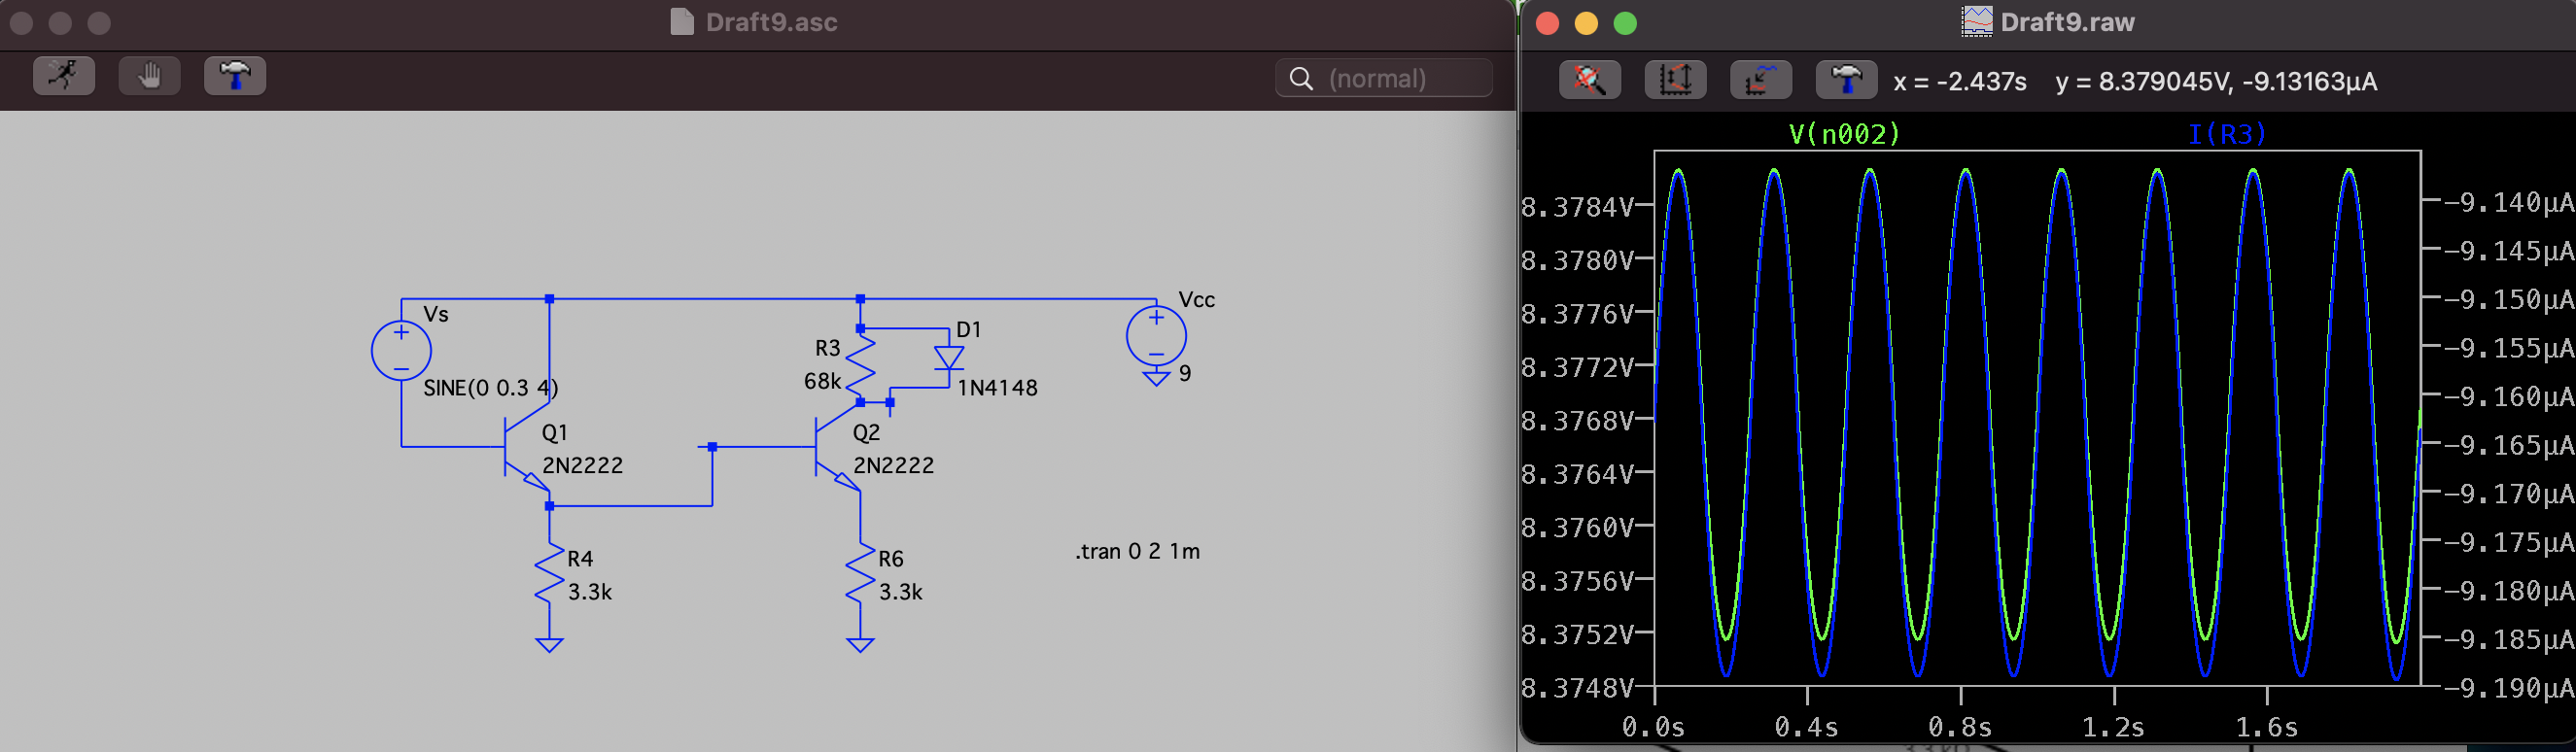
\includegraphics[width=0.8\textwidth]{Screen Shot 2021-04-19 at 7.44.28 PM.png}
\caption{{Current Through Output Resistor}}
\end{figure}

\section{Conclusion}
\indent Using two stages to amplify a very small signal (not just from a Photodiode but from any sensor) is sufficient in order for you to successfully amplify a signal. What is most important for this case is that you maintain the integrity of the signal and not attenuate it with each stage. This is a common problem in audio amplification because of improperly matched stages which result in losses. \par
\indent I was also able to create a prototype which is fully functional. I have had a 9V battery soldered onto it for a month now and it has yet to drain and be replaced, showing that this is an efficient circuit and can potentially be used for an application. IR transmitters can also be used in a similar way to send pulses of IR waves and trigger a relay or switch. This is just one way of applying the Photodiode in the real world. The following link here is to show images of the prototype and a short video showing it functioning \xrightarrow{}  \href{https://drive.google.com/drive/folders/1RGebFbM-IzBrwmx2i25E25xLZyl_BtPo?usp=sharing}{Project Folder}

\end{document}
